\section{Experimental Design}

Using the API provided by the Sloan Digital Sky Survey, we collected 2000 images consisting of 100 elliptical and 100 spiral galaxies. Additionally, we scraped around 800 images of non-celestial objects (class: invalid) to enhance our models' ability to differentiate galaxies from other objects.

Finding images of irregular galaxies was challenging. We obtained approximately 200 unique images of irregular galaxies and used data augmentation to generate 1000 images from them.

For data augmentation of irregular galaxies, we manually removed duplicate images and applied the following transformations:
\begin{itemize}
    \item ChannelShuffle (RGB to any other order) with a probability of 0.35
    \item Zoom-in and Zoom-out up to 10\%
    \item Horizontal or Vertical Flip with a probability of 0.5
    \item Rotation by 90°, 180°, 270°, or 360° with a probability of 0.5
\end{itemize}

We generated exactly 1000 images of irregular
galaxies using the above transformations. Figure 1.1
illustrates how we generate eight seemingly unique
images from just one image!

\begin{figure}[H]
    \centering
    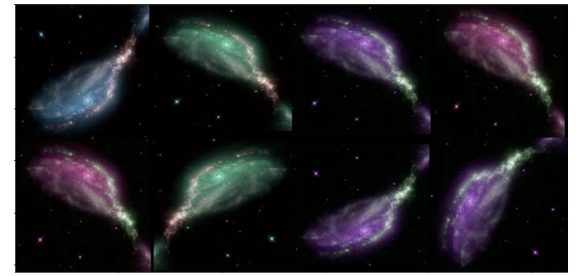
\includegraphics[width=0.5\textwidth]{Images/augmented-sample.png}
    \caption{Data-augmentation (Eight images out of one!)}
    \label{fig:enter-label}
\end{figure}

We resized all images to \(128 \times 128\) pixels and combined them into our final dataset, which includes:

\begin{itemize}
    \item 1001 Spiral images
    \item 991 Irregular images
    \item 828 Elliptical images
    \item 800 Invalid images
\end{itemize}

We applied PCA to the images for dimensionality reduction. Image preprocessing involved flattening images and Z-score normalization. Each image was represented as a vector of size \(128 \times 128 \times 3 = 49152\). The observed total variance after normalization was slightly less than the theoretical expectation (49116), confirming Hypothesis 0.1.

To preserve approximately 95\% of the variance, we determined that using 256 Principal Components (PCs) was sufficient based on the explained variance plot (Figure 1.2).

After PCA, we split the data into 70\% training and 30\% validation sets. Figures 1.3 and 1.4 illustrate sample images before and after PCA, respectively.

\begin{figure}[H]
    \centering
    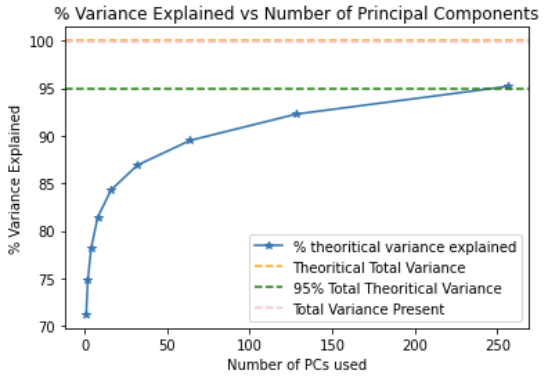
\includegraphics[width=0.5\textwidth]{Images/percent-variance.png}
    \caption{Percent of variances explained by number of Principal Components}
\end{figure}

\begin{figure}[H]
    \centering
    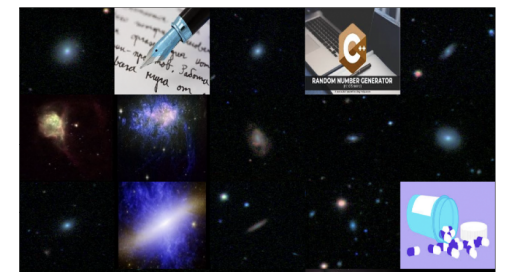
\includegraphics[width=0.5\textwidth]{Images/before-pca.png}
    \caption{Sample images before applying PCA (high dimension)}
\end{figure}

\begin{figure}[H]
    \centering
    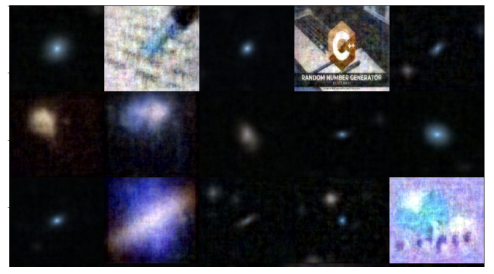
\includegraphics[width=0.5\textwidth]{Images/after-pca.png}
    \caption{Same images after applying PCA (reduced dimension)}
\end{figure}

We trained Support Vector Machine (SVM) and Random Forest classifiers on the dataset. For SVM, a linear kernel provided the highest accuracy. The Random Forest classifier used the Gini index as the split criterion with 100 trees.

We also trained a Multi-Layer Perceptron (MLP) using Keras with TensorFlow backend. Hyperparameter tuning involved selecting an adaptive momentum optimizer, dropout rate, and layer configuration. Training and validation learning curves for the MLP are shown in Figure 1.5.

\begin{figure}[H]
    \centering
    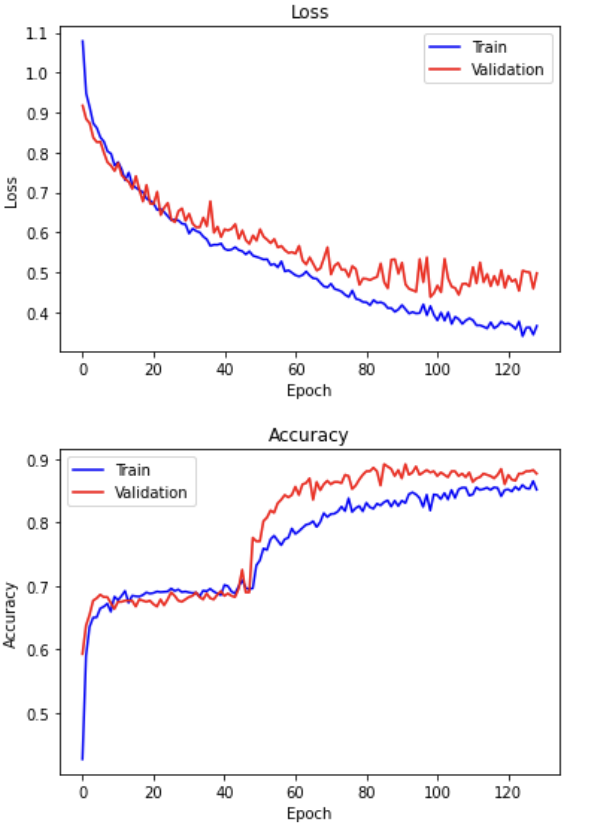
\includegraphics[width=0.5\textwidth]{Images/loss-accuracy-mlp.png}
    \caption{Loss and Accuracy plots generated for training and validation in MLP}
\end{figure}

Similarly, we trained a Convolutional Neural Network (CNN) with optimized hyperparameters. The best-performing CNN model had 4 layers with rectified linear activation and achieved training and validation accuracy depicted in Figure 1.6.
